\documentclass[a4paper]{article}
\usepackage[english]{babel}
\usepackage{multicol}
\usepackage{amsmath}
\usepackage{amsfonts}
\usepackage{amssymb}
\usepackage[font=scriptsize]{caption}
\usepackage{parskip}
\usepackage[a4paper, margin=1in, total={6in, 8in}]{geometry}
\usepackage{titling}
\usepackage{subcaption}
\usepackage{float}
\usepackage{placeins}
\usepackage{graphicx}

\parskip = 6pt plus 2pt minus 2pt
\setlength{\droptitle}{-2cm}

\title{HW8 - Computer Simulation II}
\author{Schewtschik, Guilherme (3748052)}
\date{\today}

\begin{document}
\maketitle

\section{}
Given that beta and L are related by the equation:
\begin{equation}
    \beta = a+ \frac{b}{L^2}
\end{equation}

It is best to work with the variable $\tilde{L} = 1/L^2$, and then convert it back to $L$. Fitting $a$ and $b$ for $L_{min} = 8$ we get the following graph:

\begin{figure}[ht]
    \centering
    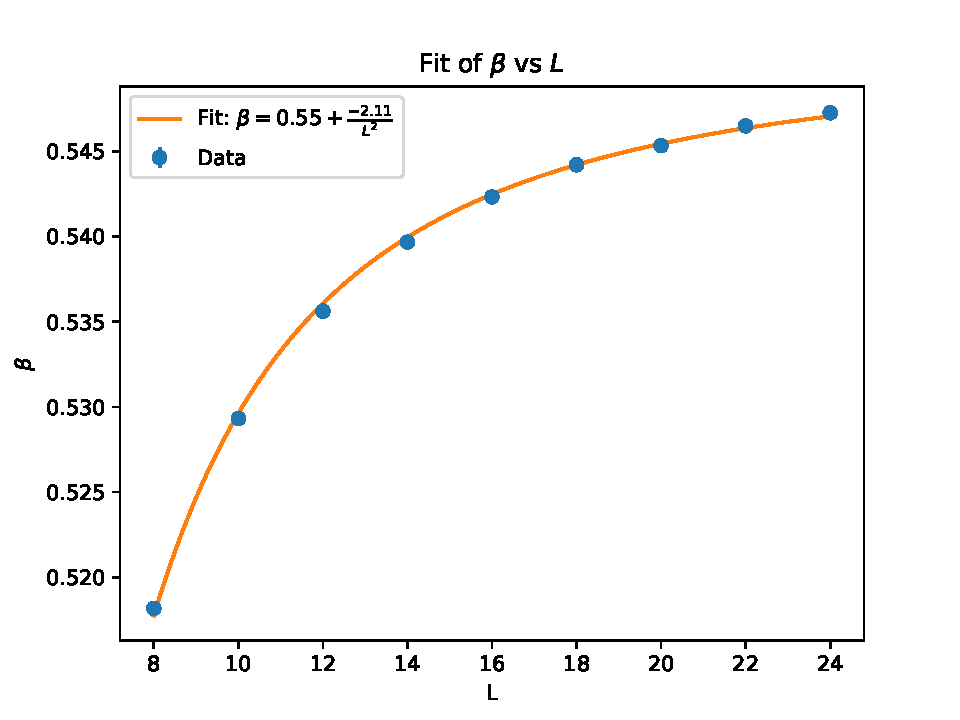
\includegraphics[width=0.7\textwidth]{figures/beta_fit.pdf}
\end{figure}

We can see that the fit is at a first glance good but deviates in some points, lets calculate the relative error of the individual points and $\chi^2/(N-2)$:
\[
    \frac{\chi^2}{N-2} \approx 10.44
\]
 

\begin{table}[ht]
\centering
\renewcommand{\arraystretch}{1.3}

\begin{tabular}{|c|c|c|}
\hline
$\beta$ & $\beta_{\mathrm{fit}}$ & Relative Error \\
\hline
0.51818 & 0.51776 & 4.22 \\
0.52932 & 0.52962 & -3.03 \\
0.53562 & 0.53607 & -4.07 \\
0.53967 & 0.53995 & -2.84 \\
0.54232 & 0.54248 & -1.95 \\
0.54421 & 0.54421 & 0.05 \\
0.54533 & 0.54544 & -1.41 \\
0.54649 & 0.54636 & 2.64 \\
0.54726 & 0.54705 & 2.94 \\
\hline
\end{tabular}
\renewcommand{\arraystretch}{1}
\caption{Fit results for all lattice sizes $L=8,\ldots,24$.}

\end{table}

Given that the ansatz expects $\chi^2/(N-2) \approx 1$, the fit quality is poor for $L_{\min} = 8$, now ranging over $L_{min}$
values we can find the optimal range of $L$ values to fit the data:

\begin{table}[ht]
\centering
\renewcommand{\arraystretch}{1.3}
\begin{tabular}{|c|c|c|c|c|}
\hline
$L_{\min}$ & $N$ & $a$ & $b$ & $\chi^2/\mathrm{dof}$ \\
\hline
8  & 9 & 0.550716 & -2.109338 & 10.443 \\
10 & 8 & 0.550936 & -2.181172 &  2.859 \\
12 & 7 & 0.551079 & -2.234493 &  1.143 \\
14 & 6 & 0.551122 & -2.251716 &  1.268 \\
16 & 5 & 0.551162 & -2.269470 &  1.584 \\
18 & 4 & 0.551242 & -2.307417 &  2.210 \\
\hline
\end{tabular}
\renewcommand{\arraystretch}{1}

\caption{Weighted fits for different lower cutoffs $L_{\min}$.}
\label{tab:lmin_fits}
\end{table}

\newpage
So for $L_{min} = 12$ we get the best fit, with $\chi^2/(N-2) \approx 1.143$, and the fit parameters are $a \approx 0.55$ and $b \approx -2.23$. This means that the critical beta value in the thermodynamic limit is approximately $\beta_c \approx 0.551079$.

\section{}
Rewrite the equation in a logarithmic form:
\[
    \ln(\chi(\beta)) = -\gamma \ln(a) - \gamma \ln(1-\beta/\beta_c)
\]

Fitting the curve in log space for $\beta \in [0.99, 0.85]\beta_c$ and taking into account the error $e_{\ln(\chi)} = \sigma/\chi$, where sigma is the standard deviation from cluster size, we get the following plots.

\begin{figure}[ht]
    \centering
    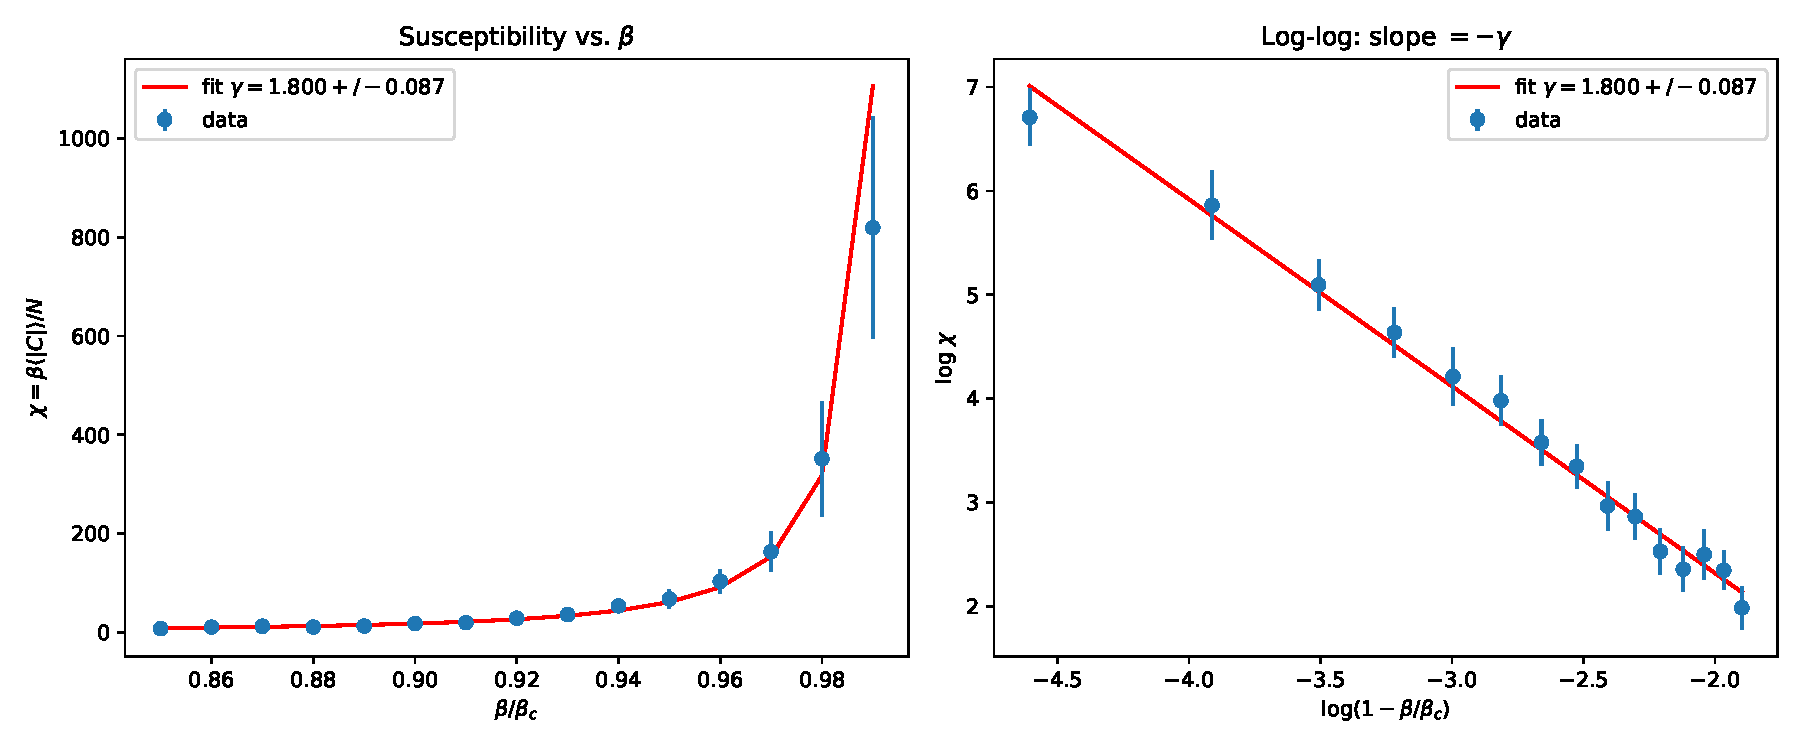
\includegraphics[width=0.7\textwidth]{figures/chi_beta_norm.pdf}
\end{figure}

The values for $\gamma = 1.80 \pm 0.087$ is well in the theoretical expectation of $\gamma = 1.75$ for the 2D Ising model.

\end{document}
